%-------------------------------------------------------------------------
% corriges-ds-info-S1-boucles-imbriquees.tex
%-------------------------------------------------------------------------

%-------------------------------------------------------------------------
\documentclass[11pt,a4paper]{article}
%-------------------------------------------------------------------------

%-------------------------------------------------------------------------
\input{corriges-ds-info-S1-preambule.tex}
%-------------------------------------------------------------------------

%-------------------------------------------------------------------------
\begin{document}
%-------------------------------------------------------------------------
$$\mbox{\textbf{\large Motifs géométriques}}$$


\paragraph{Questions :} 
En utilisant les instructions de la tortue \logo{}
(module \texttt{turtle}), écrire un algorithme qui dessine un motif géométrique
composé de $(n\times m)$ pavés élémentaires disposés régulièrement sur une grille
ou disposés en quinconce sur la grille.
\vspace*{3mm}

\paragraph{Réponses :} 
D'une manière générale, le code aura la structure suivante selon que les pavés sont alignés ou en quinconce :

\noindent
\mbox{}\hfill
\begin{minipage}[t]{6cm}
alignés :\\
\centerline{\includegraphics[width=3cm]{grille-1.pdf}}

\footnotesize
\begin{Verbatim}[frame=single]
# initialisation du motif
dx, dy = 20, 20
n, m = 5, 4
x0, y0 = 0, 0
# dessin du motif
for j in range(m) :
    xl = x0
    yl = y0 + j*dy
    # dessin d'une ligne de figures
    for i in range(n) :
        x, y = xl + i*dx, yl
        # dessin d'une figure
        up()
        goto(x,y)
        setheading(0)
        down()
        # tracé de la figure
\end{Verbatim}
\end{minipage}
\hfill
\begin{minipage}[t]{6cm}
en quinconce :\\
\centerline{\includegraphics[width=3cm]{grille-2.pdf}}

\footnotesize
\begin{Verbatim}[frame=single]
# initialisation du motif
dx, dy = 20, 20
n, m = 5, 4
x0, y0 = 0, 0
# dessin du motif
for j in range(m) :
    xl = x0 + dx*(j%2)/2
    yl = y0 + j*dy
    # dessin d'une ligne de figures
    for i in range(n) :
        x, y = xl + i*dx, yl
        # dessin d'une figure
        up()
        goto(x,y)
        setheading(0)
        down()
        # tracé de la figure
\end{Verbatim}
\end{minipage}
\hfill

\vspace*{5mm}

%1,2
\noindent\begin{minipage}[t]{5cm}
\begin{enumerate}\setcounter{enumi}{0}
\item \begin{minipage}{1.75cm}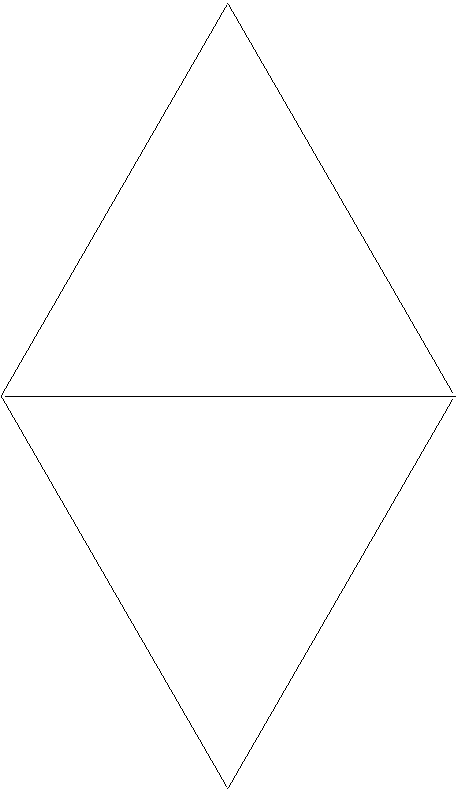
\includegraphics[height=0.75cm]{losange-2.pdf}\end{minipage} alignés
\item \begin{minipage}{1.75cm}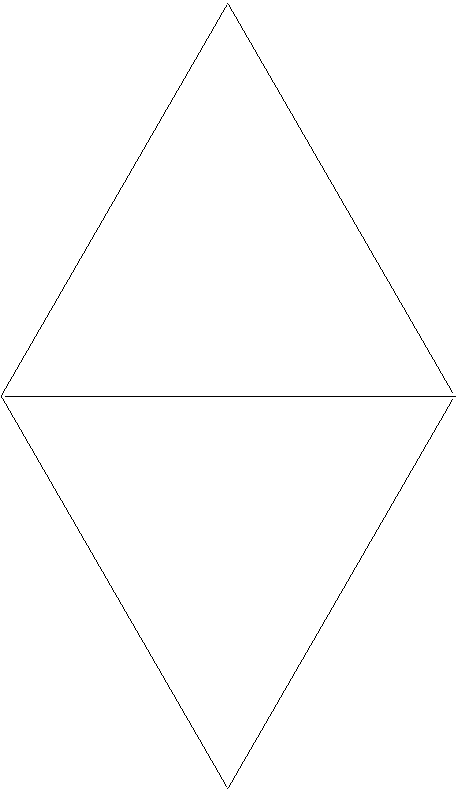
\includegraphics[height=0.75cm]{losange-2.pdf}\end{minipage} en quinconce
\end{enumerate}
\end{minipage}
\hfill
\begin{minipage}[t]{7cm}\footnotesize
\begin{Verbatim}
# tracé de la figure
c, d = 3, dx/2
for k in range(c) :
    forward(d)
    left(360/c)
for k in range(c) :
    forward(d)
    right(360/c)
\end{Verbatim}
\end{minipage}
\vspace*{5mm}

%3,4
\noindent\begin{minipage}[t]{5cm}
\begin{enumerate}\setcounter{enumi}{2}
\item \begin{minipage}{1.75cm}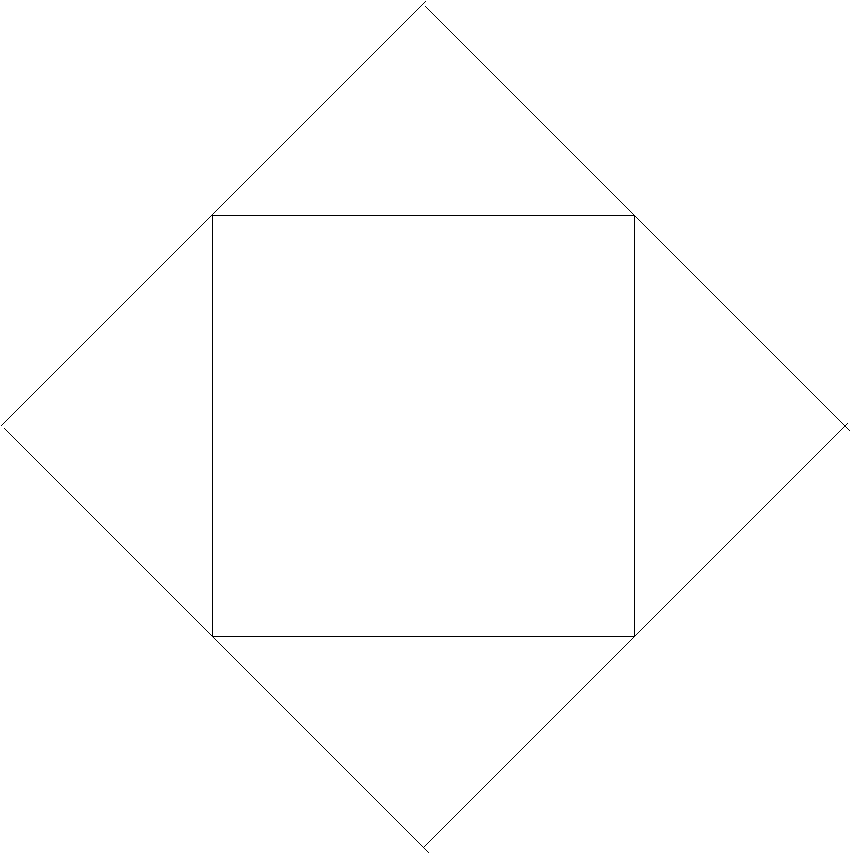
\includegraphics[height=0.75cm]{carre-2.pdf}\end{minipage} alignés
\item \begin{minipage}{1.75cm}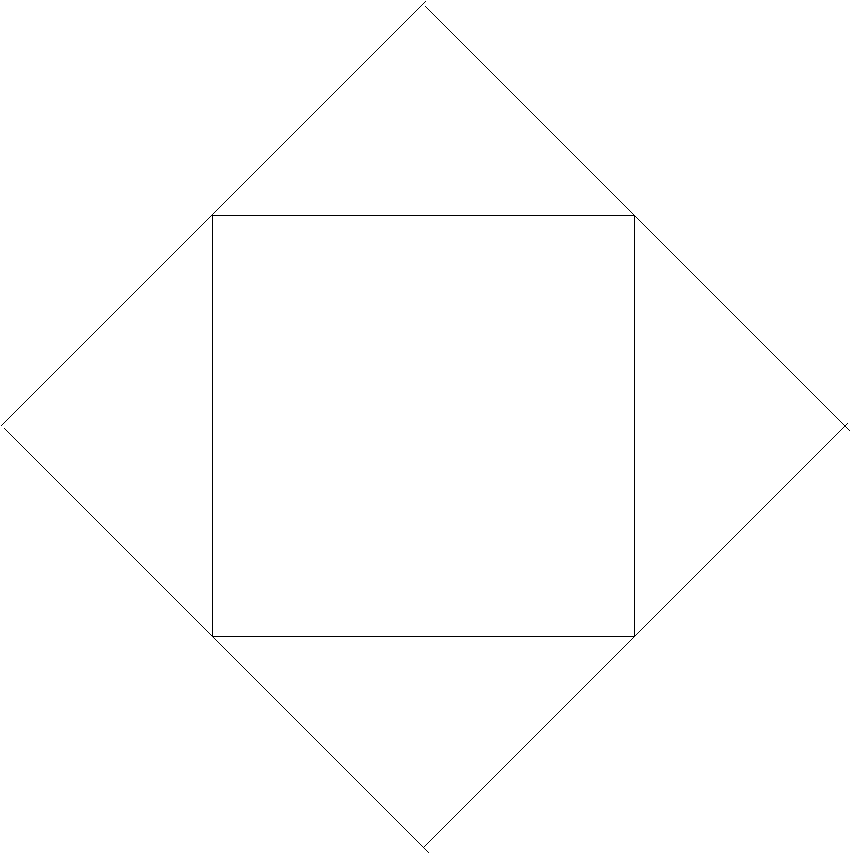
\includegraphics[height=0.75cm]{carre-2.pdf}\end{minipage} en quinconce
\end{enumerate}
\end{minipage}
\hfill
\begin{minipage}[t]{7cm}\footnotesize
\begin{Verbatim}
# tracé de la figure
c, d = 4, dx/2
for k in range(c) :
    forward(d)
    left(360/c)
up()
goto(x+d/2,y-d/2)
setheading(45)
down()
for k in range(c) :
    forward(d*sqrt(2))
    left(360/c)
\end{Verbatim}
\end{minipage}
\newpage

%5,6
\noindent\begin{minipage}[t]{5cm}
\begin{enumerate}\setcounter{enumi}{4}
\item \begin{minipage}{1.75cm}\includegraphics[height=0.75cm]{etoile-2.pdf}\end{minipage} alignés
\item \begin{minipage}{1.75cm}\includegraphics[height=0.75cm]{etoile-2.pdf}\end{minipage} en quinconce
\end{enumerate}
\end{minipage}
\hfill
\begin{minipage}[t]{7cm}\footnotesize
\begin{Verbatim}
# tracé de la figure
c, d = 3, dx/2
setheading(30)
for k in range(c) :
    forward(d)
    left(360/c)
up()
goto(x+d/sqrt(3),y)
setheading(90)
down()
for k in range(c) :
    forward(d)
    left(360/c)
\end{Verbatim}
\end{minipage}
\vspace*{5mm}


%7,8
\noindent\begin{minipage}[t]{5cm}
\begin{enumerate}\setcounter{enumi}{6}
\item \begin{minipage}{1.75cm}\includegraphics[height=0.75cm]{cercle-2.pdf}\end{minipage} alignés
\item \begin{minipage}{1.75cm}\includegraphics[height=0.75cm]{cercle-2.pdf}\end{minipage} en quinconce
\end{enumerate}
\end{minipage}
\hfill
\begin{minipage}[t]{7cm}\footnotesize
\begin{Verbatim}
# tracé de la figure
c, d = 3, dx/2
for k in range(c) :
    forward(d)
    left(360/c)
setheading(-60)
circle(d/sqrt(3))
\end{Verbatim}
\end{minipage}
\vspace*{5mm}


%9,10
\noindent\begin{minipage}[t]{5cm}
\begin{enumerate}\setcounter{enumi}{8}
\item \begin{minipage}{1.75cm}\includegraphics[height=0.75cm]{hexagone-2.pdf}\end{minipage} alignés
\item \begin{minipage}{1.75cm}\includegraphics[height=0.75cm]{hexagone-2.pdf}\end{minipage} en quinconce
\end{enumerate}
\end{minipage}
\hfill
\begin{minipage}[t]{7cm}\footnotesize
\begin{Verbatim}
# tracé de la figure
c, d = 3, dx/2
for n in range(6) :
    setheading(n*60)
    for k in range(c) :
        forward(d)
        left(360/c)
\end{Verbatim}
\end{minipage}
\vspace*{5mm}


%11,12
\noindent\begin{minipage}[t]{5cm}
\begin{enumerate}\setcounter{enumi}{10}
\item \begin{minipage}{1.75cm}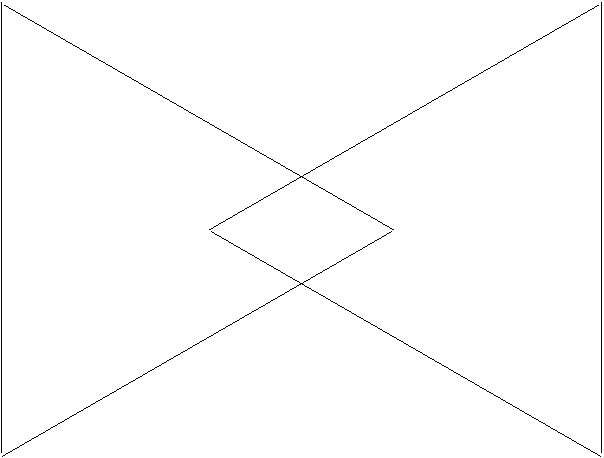
\includegraphics[height=0.75cm]{triangle-2.pdf}\end{minipage} alignés
\item \begin{minipage}{1.75cm}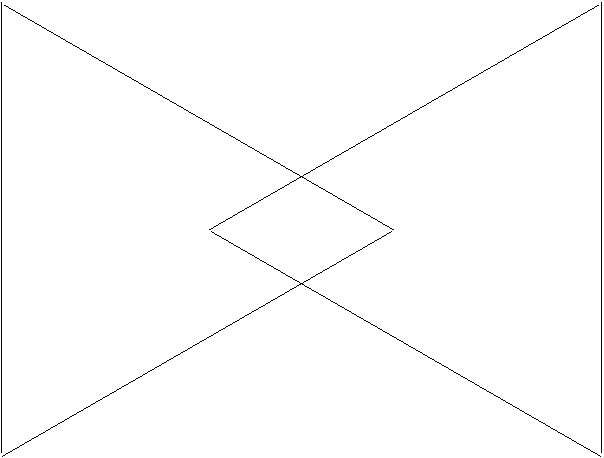
\includegraphics[height=0.75cm]{triangle-2.pdf}\end{minipage} en quinconce
\end{enumerate}
\end{minipage}
\hfill
\begin{minipage}[t]{7cm}\footnotesize
\begin{Verbatim}
# tracé de la figure
c, d = 3, dx/2
setheading(30)
for k in range(c) :
    forward(d)
    left(360/c)
up()
goto(x+d/sqrt(3),y+d/2)
setheading(-30)
down()
for k in range(c) :
    forward(d)
    left(360/c)
\end{Verbatim}
\end{minipage}
\vspace*{5mm}

%13,14
\noindent\begin{minipage}[t]{5cm}
\begin{enumerate}\setcounter{enumi}{12}
\item \begin{minipage}{1.75cm}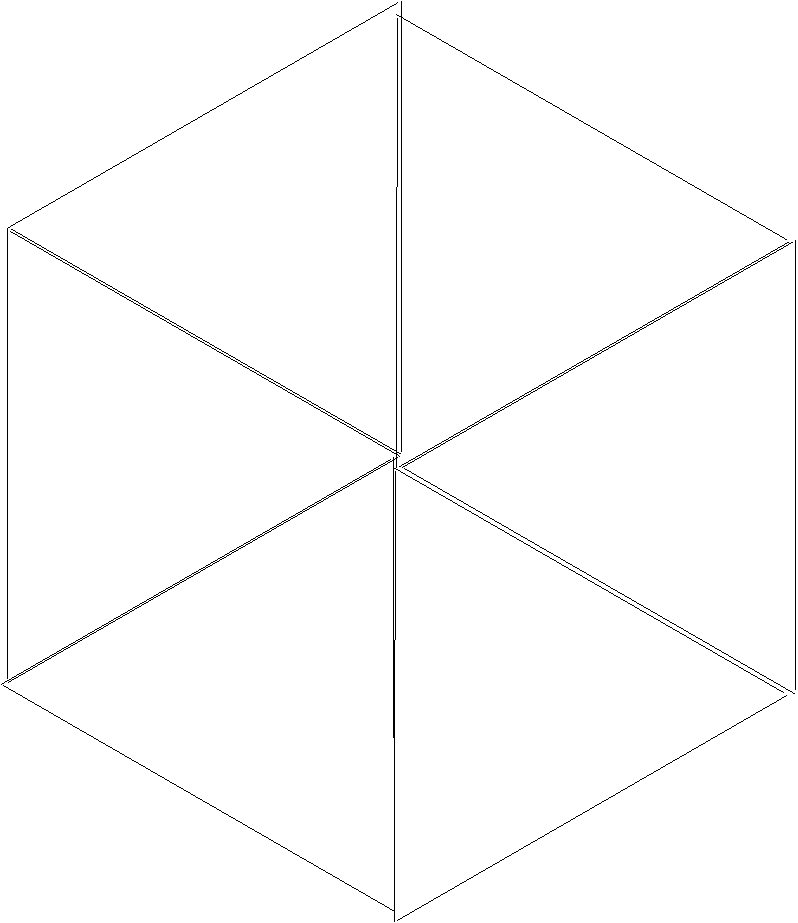
\includegraphics[height=0.75cm]{hexagone-1.pdf}\end{minipage} alignés
\item \begin{minipage}{1.75cm}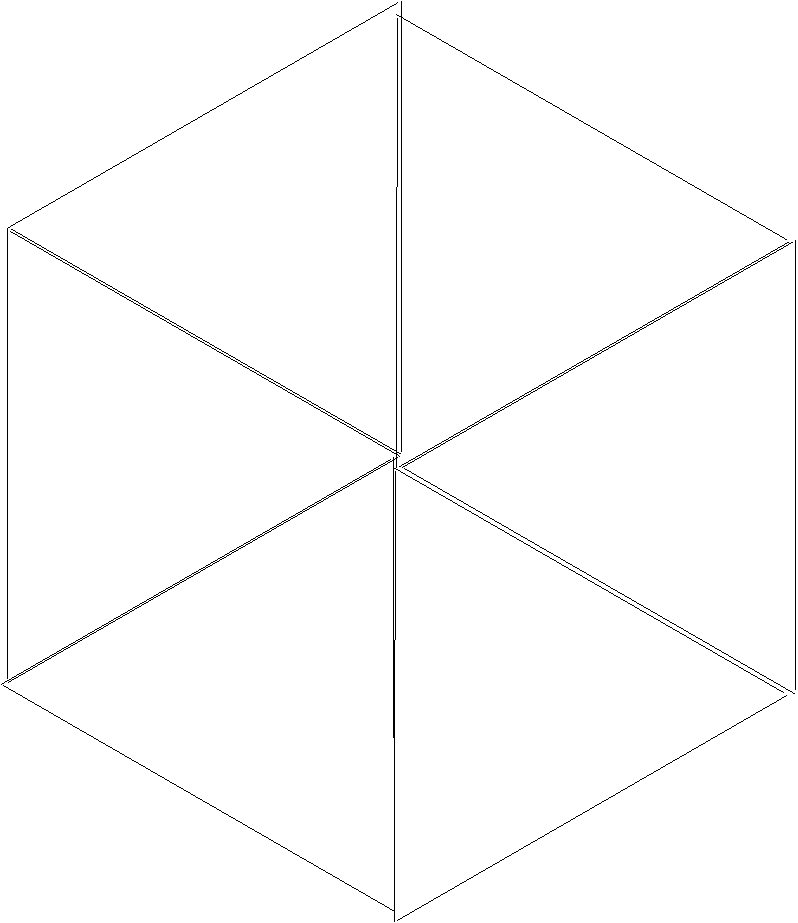
\includegraphics[height=0.75cm]{hexagone-1.pdf}\end{minipage} en quinconce
\end{enumerate}
\end{minipage}
\hfill
\begin{minipage}[t]{7cm}\footnotesize
\begin{Verbatim}
# tracé de la figure
c, d = 3, dx/2
for n in range(6) :
    setheading(30+n*60)
    for k in range(c) :
        forward(d)
        left(360/c)
\end{Verbatim}
\end{minipage}
\vspace*{5mm}

\newpage
%15,16
\noindent\begin{minipage}[t]{5cm}
\begin{enumerate}\setcounter{enumi}{14}
\item \begin{minipage}{1.75cm}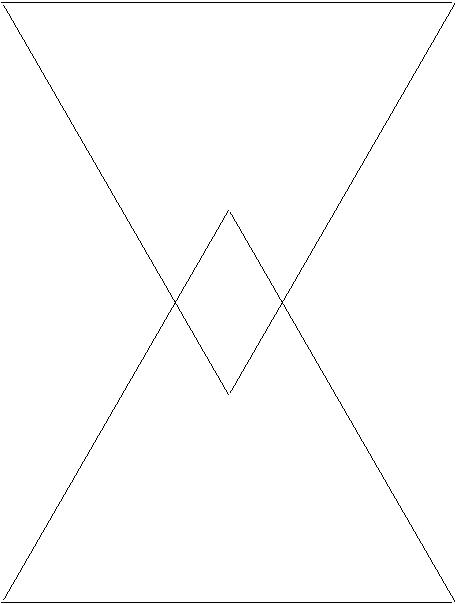
\includegraphics[height=0.75cm]{triangle-1.pdf}\end{minipage} alignés
\item \begin{minipage}{1.75cm}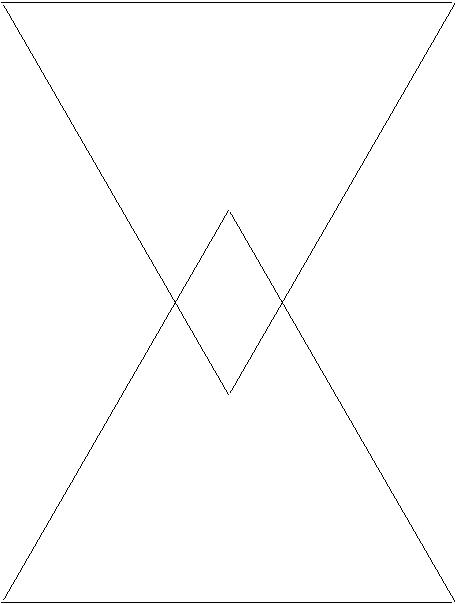
\includegraphics[height=0.75cm]{triangle-1.pdf}\end{minipage} en quinconce
\end{enumerate}
\end{minipage}
\hfill
\begin{minipage}[t]{7cm}\footnotesize
\begin{Verbatim}
# tracé de la figure
c, d = 3, dx/2
for k in range(c) :
    forward(d)
    left(360/c)
up()
goto(x+d/2,y+d/sqrt(3))
setheading(60)
down()
for k in range(c) :
    forward(d)
    left(360/c)
\end{Verbatim}
\end{minipage}
\vspace*{5mm}

%17,18
\noindent\begin{minipage}[t]{5cm}
\begin{enumerate}\setcounter{enumi}{16}
\item \begin{minipage}{1.75cm}\includegraphics[height=0.75cm]{losange-1.pdf}\end{minipage} alignés
\item \begin{minipage}{1.75cm}\includegraphics[height=0.75cm]{losange-1.pdf}\end{minipage} en quinconce
\end{enumerate}
\end{minipage}
\hfill
\begin{minipage}[t]{7cm}\footnotesize
\begin{Verbatim}
# tracé de la figure
c, d = 3, dx/2
setheading(30)
for k in range(c) :
    forward(d)
    left(360/c)
setheading(90)
for k in range(c) :
    forward(d)
    left(360/c)
\end{Verbatim}
\end{minipage}
\vspace*{5mm}

%19,20
\noindent\begin{minipage}[t]{5cm}
\begin{enumerate}\setcounter{enumi}{18}
\item \begin{minipage}{1.75cm}\includegraphics[height=0.75cm]{carre-1.pdf}\end{minipage} alignés
\item \begin{minipage}{1.75cm}\includegraphics[height=0.75cm]{carre-1.pdf}\end{minipage} en quinconce
\end{enumerate}
\end{minipage}
\hfill
\begin{minipage}[t]{7cm}\footnotesize
\begin{Verbatim}
# tracé de la figure
c, d = 4, dx/2
for k in range(c) :
    forward(d)
    left(360/c)
up()
goto(x+d/2,y)
setheading(45)
down()
for k in range(c) :
    forward(d/sqrt(2))
    left(360/c)
\end{Verbatim}
\end{minipage}
\vspace*{5mm}

%21,22
\noindent\begin{minipage}[t]{5cm}
\begin{enumerate}\setcounter{enumi}{20}
\item \begin{minipage}{1.75cm}\includegraphics[height=0.75cm]{etoile-1.pdf}\end{minipage} alignés
\item \begin{minipage}{1.75cm}\includegraphics[height=0.75cm]{etoile-1.pdf}\end{minipage} en quinconce
\end{enumerate}
\end{minipage}
\hfill
\begin{minipage}[t]{7cm}\footnotesize
\begin{Verbatim}
# tracé de la figure
c, d = 3, dx/2
for k in range(c) :
    forward(d)
    left(360/c)
up()
goto(x,y+d/sqrt(3))
down()
for k in range(c) :
    forward(d)
    right(360/c)
\end{Verbatim}
\end{minipage}
\vspace*{5mm}

%23,24
\noindent\begin{minipage}[t]{5cm}
\begin{enumerate}\setcounter{enumi}{22}
\item \begin{minipage}{1.75cm}\includegraphics[height=0.75cm]{cercle-1.pdf}\end{minipage} alignés
\item \begin{minipage}{1.75cm}\includegraphics[height=0.75cm]{cercle-1.pdf}\end{minipage} en quinconce
\end{enumerate}
\end{minipage}
\hfill
\begin{minipage}[t]{7cm}\footnotesize
\begin{Verbatim}
# tracé de la figure
c, d = 3, dx/2
for k in range(c) :
    forward(d)
    right(360/c)
setheading(-120)
circle(d/sqrt(3))
\end{Verbatim}
\end{minipage}
%\vspace*{5mm}


%-------------------------------------------------------------------------
\end{document}
%-------------------------------------------------------------------------
